\documentclass[a4paper,12pt]{article}

\usepackage{rotating}
\usepackage[top=1.25in, bottom=1.25in, left=1.0in, right=1.03in]{geometry}
\usepackage{graphicx}
\usepackage[numbers,square,sort&compress]{natbib}
\usepackage{setspace}
\usepackage[cdot,mediumqspace,]{SIunits}
\usepackage{caption}
\usepackage{subcaption}
\usepackage{mathtools}
\usepackage{authblk}
\usepackage{float}
\usepackage{wrapfig}
\renewcommand{\thesubsection}{\thesection.\alph{subsection}}
\providecommand{\e}[1]{\ensuremath{\times 10^{#1}}}
\newcommand*\lap{\mathop{}\!\mathbin\bigtriangleup}

\begin{document}
%\onehalfspacing
\title{Lab Report: Special Functions and Solving the Heat Equation for a Cold Cylinder}
\author{Natalie Price-Jones, 999091021}
\date{4 December 2014}
\affil{\small{natalie.price.jones@mail.utoronto.ca}}
\maketitle

\section{Question 1}
\begin{table}[H]
  \centering
  \begin{tabular}{|c||c||c||c||c|}
    \hline
    Factorial & math.factorial & Recursive & Stirling & Memoization\\
    \hline
    \hline
    10! & $3.0\e{-6}$ s & $2.2\e{-5}$ s & $8.0\e{-6}$ s & $3.7\e{-6}$ s\\
    \hline
    100! & $1.6\e{-5}$ s & $2.1\e{-4}$ s& $1.0\e{-6}$ s& $4.0\e{-6}$s\\
    \hline
    500! & $1.2\e{-4}$ s& $1.0\e{-3}$ s& Overflowed & $2.2\e{-5}$ s\\
    \hline
    1000! & $5.0\e{-4}$ s& Recursion exceeded & Overflowed & $3.9\e{-5}$s\\
    \hline
  \end{tabular}
  \caption{A comparison of the speed of computing several factorials in seconds.}
\end{table}

It is obvious from this table that math.factorial is consistently faster than the recursion method. This is because the math module relies on precomplied C libraries, inherently faster to run than interpreted languages like Python. In addition, math.factorial uses a divide and conquer method to compute factorials, reducing the time needed to evaluate. However, the Stirling approximation and the memoization method both beat it for time.

When my first recursive function attempted to evaluate 1000!, it failed because it exceeded the maximum recursion depth allowed for a recursive function. Essentially, it went too many layers into itself. Initially memoization has the same problem, though of course once a sufficient number of lower factorials were saved, evaluating 1000! did not exceed the recursion depth. The Stirling approximation was one of the faster methods, but it was only successful in evaluation $\ln(1000!)$. This value could not be converted back to 1000! without an overflow error. In addition, the advantage of the speed of the Stirling approximation was somewhat negated by the fact that it is only an approximation, and does not work well for small factorials. Although it gets an answer fast, it is not necessarily the right answer.

\textbf{part b)} $\ln(1000!)$ is about 0.07 \% different from math.log(math.factorial(1000!). As we might expect, $\ln(1\e{5}!)$ is computed much more quickly with Stirling's approximation, and the percentage difference between the two results is now $0.0006$ \%.

\textbf{part c)} One obvious advantage of memoization to compute factorials is that it extends the capabilities of our recursive function far beyond its normal range. However, these results are lost when the program is restarted, so the memoized data must be reevaluated each time the program is run. This shortcoming could be overcome by saving the results of the factorial computation and reading them in each time the program starts, appending new values to the end of the file as they are computed. This would overcome the obvious disadvantage of memoization and add only a short slow-down when the file is loaded in.

\textbf{part d)} For the remainder of the coding, I will be using the memoization function, as it is by far the fastest and can be used to evaluate larger factorials.

\section{Question 2}

\textbf{part b)}

As we can see in Figure \ref{fig:q2b}, an increasing number of terms improves the accuracy of the curve.

\begin{figure}[H]
\centering
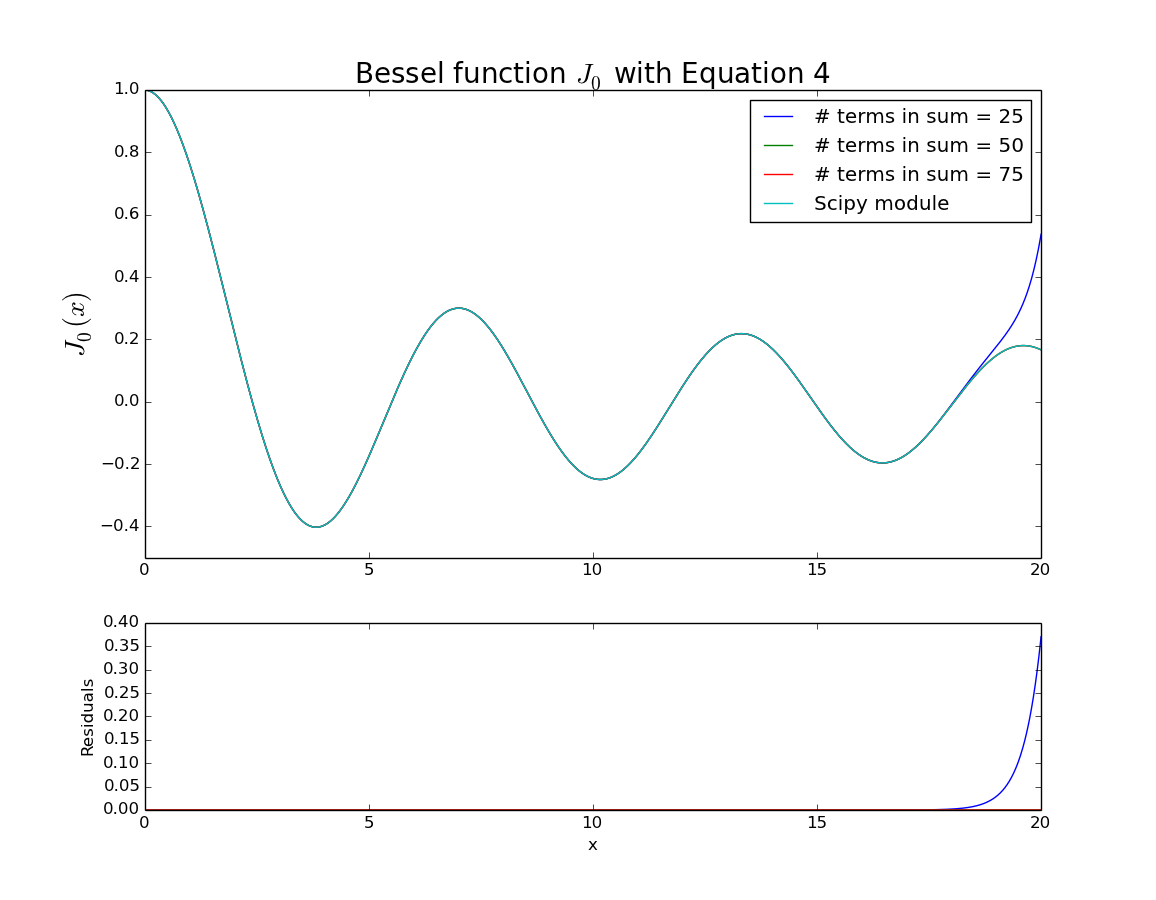
\includegraphics[width = 0.8\linewidth]{indepq2b.png}
\caption{}
\label{fig:q2b}
\end{figure}

\textbf{part c)}

As the x-range is increased to make Figure \ref{fig:q2c}, each curve becomes far less accurate at the maximal x point. This is because as we go further from zero, we need more terms in the sum to get the true result.

\begin{figure}[H]
\centering
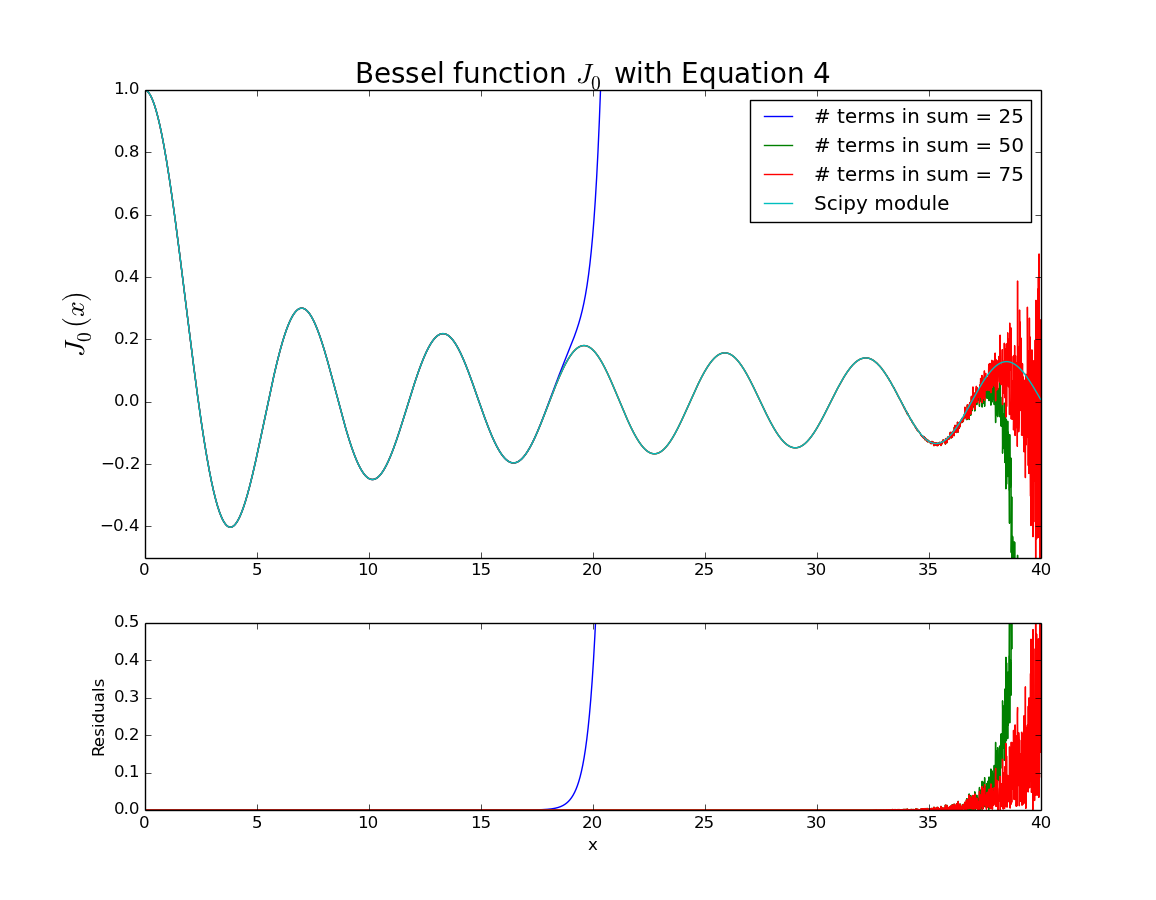
\includegraphics[width = 0.8\linewidth]{indepq2c.png}
\caption{}
\label{fig:q2c}
\end{figure}

\textbf{part d)}

\begin{figure}[H]
\centering
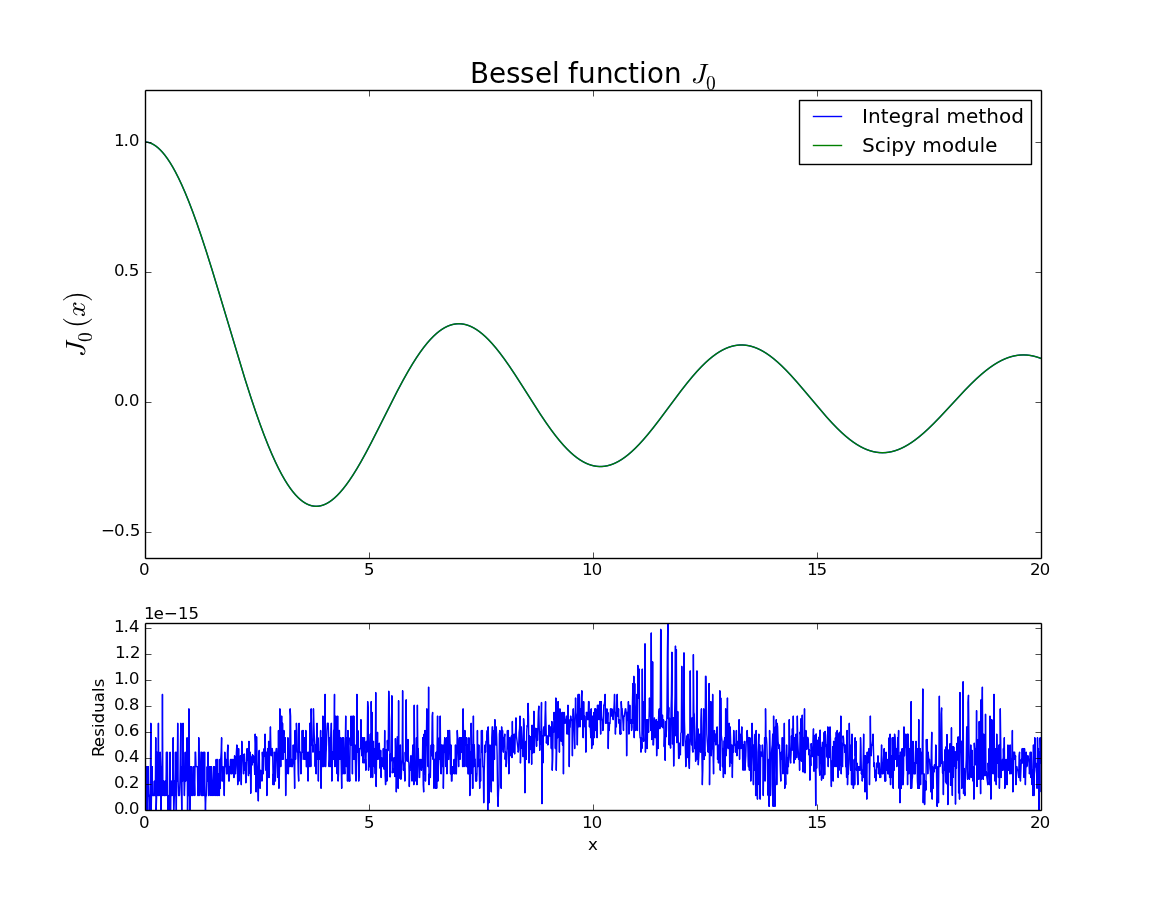
\includegraphics[width = 0.8\linewidth]{indepq2d.png}
\caption{Using the integral method to create plot above matches the scipy curve very closely.}
\label{fig:q2d}
\end{figure}

\textbf{part e)} For the remainder of the code, I plan to use the integral equation for the Bessel function:

\begin{equation}
J_n(x) = \frac{1}{\pi}\int_0^{\pi}\cos(n\tau - x\sin(\tau)) d\tau,\nonumber
\end{equation} 
%
since this is quicker and easier to evaluate than an arbitrarily large sum, and matches our expected result (the scipy module) very well.

\textbf{part f)}

\begin{figure}[H]
\centering
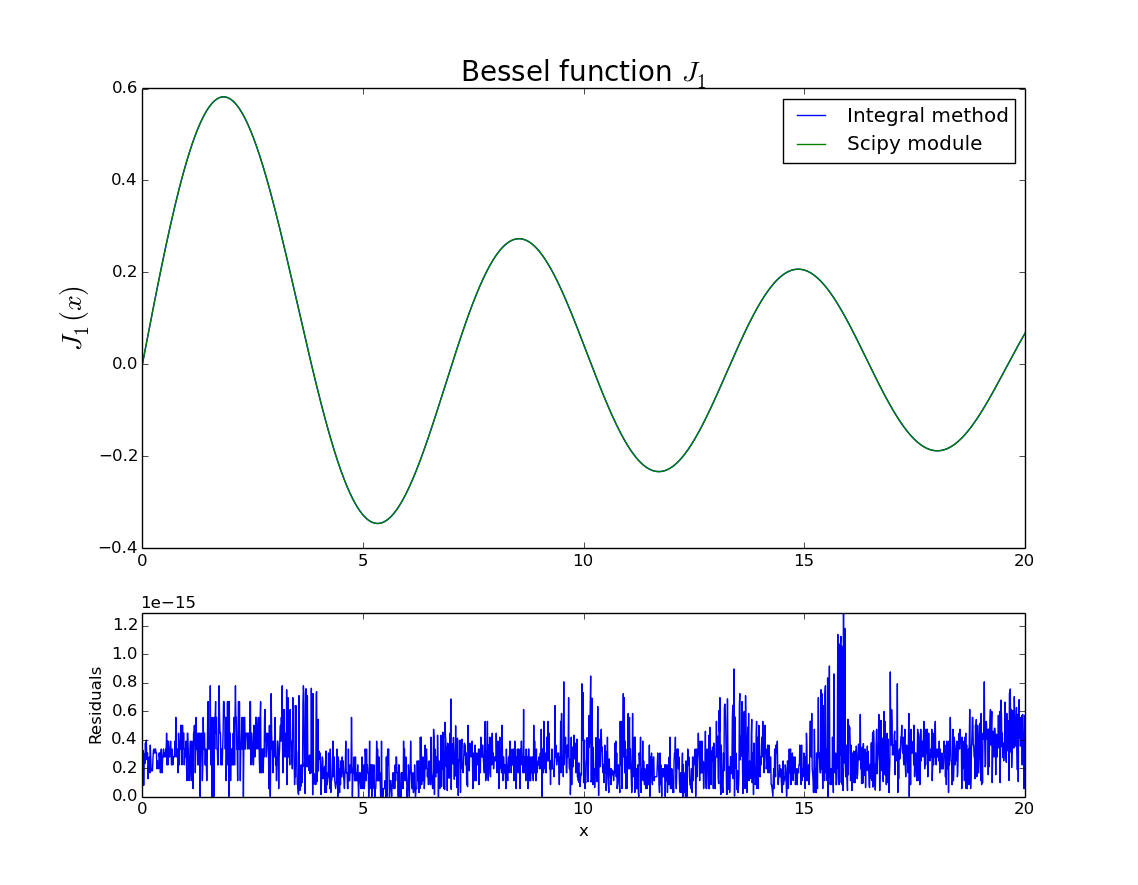
\includegraphics[width = 0.8\linewidth]{indepq2f.png}
\caption{}
\label{fig:q2f}
\end{figure}

\section{Question 3}

\textbf{part a)}

I chose to use the secant method. The required accuracy to match the first five zeros was $1\e{-5}$.\\

\textbf{part b)}

\begin{table}[H]
  \centering
  \begin{tabular}{|c||c||c|c|}
    \hline
    Zero Index & Approximation Scheme & scipy.special.jn\_zeros & Difference\\
    \hline
    \hline
    5 & 14.9226 & 14.9309 & $8.3\e{-3}$\\
    \hline
    50 & 156.2942 & 156.2950 & $7\e{-4}$\\
    \hline
    500 & 1570.0109 & 1570.0110 & $8\e{-5}$\\
    \hline
  \end{tabular}
\end{table}

The value for the 5th zero matches the result from part a) only two three significant figure. Obviously our approximation is best for large values of the zero index.

\section{Question 4} 

\begin{figure}[H]
\centering
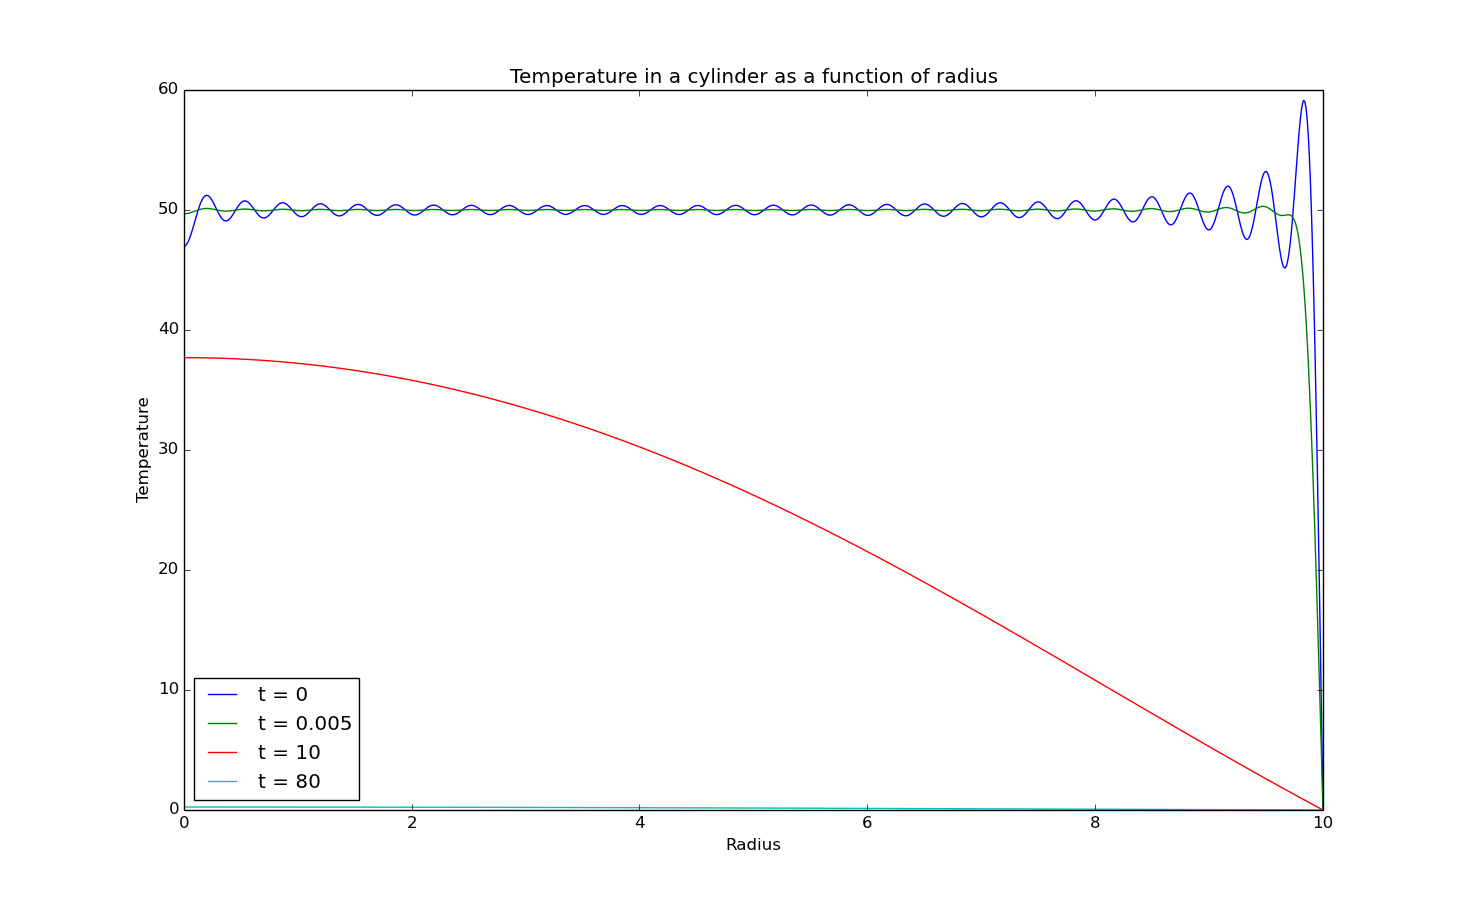
\includegraphics[width = 0.8\linewidth]{indepq4.png}
\caption{}
\label{fig:q4}
\end{figure}

At time 0, the temperature profile does not obey the initial conditions of the problem. This is because we are forced to truncate the solution to a finite number of terms in the sum. We are trying to use an oscillatory function to model a step function. We saw this exact sort of problem in a past lab when we tried to model a square wave with a Fourier series. We could reduce the oscillations by increasing the number of terms in the sum, although this has the effect of increasing the size of the spike near the edge of the cylinder.

Obviously there is some additional uncertainty in our result related to the accuracy of our zero finding method and integration technique. We have already seen that Gaussian integration tends to be very accurate. Our results in Question 2 for parts d) and f) show that the evaluation of $J_0$ and $J_1$ differ from the expected results by numbers on order of the machine precision ($\sim 1\e{-15}$). The zero finding method matches scipy.special.jn\_zeros quite well for lower order zeros, but errors begin to increase as more numbers are computing, ending up with differences on order $1\e{-5}$ even after the tolerance was decreased to $1\e{-9}$. This is strange, given that the actual function the zero finder is working on matches the expected result so well. However, switching to using scipy.special.jn\_zeros to find the $\lambda_n$s offered no improvement. It seems the dominant factor on the $t = 0$ shape is in fact the number of terms in the sum.

However unexpected the shape may be at t = 0, we can see in Figure \ref{fig:q4} that by t = 0.005, the shape is almost exactly how we would expect it, with oscillations minimized. As time goes on, the function smooths out to be exactly what we would expect. Further more, the total temperature decreases everywhere over time as expected, with low temperature regions moving inward from the outer edge where the temperature is fixed.


\end{document}
